\documentclass[11pt]{article}

\usepackage[margin=1in]{geometry}
\usepackage{amsmath}
\usepackage{amssymb}
\usepackage{booktabs}
\usepackage{graphicx}
\usepackage{microtype}
\usepackage[round]{natbib}
\usepackage{xcolor}
\usepackage{xspace}
\usepackage{hyperref}

\graphicspath{{figures/}}

\newcommand{\dreems}{DREEMS\xspace}
\newcommand{\feems}{FEEMS\xspace}
\newcommand{\vect}[1]{\boldsymbol{#1}}

\title{Deep recovery of effective migration surfaces}
\author{Jonathan Terhorst\\
Department of Statistics, University of Michigan}
\date{}

\begin{document}
\maketitle

\begin{abstract}
Spatial population genetic data often exhibit isolation by distance, but the
rate at which genetic similarity decays can vary across a habitat. EEMS and
\feems visualize this heterogeneity as a surface of relative effective
migration. \feems obtains a surface by penalized optimization and selects its
spatial regularization separately for each dataset, which can require many
fits. Here we introduce Deep Resistance Estimation of Effective Migration
Surfaces (\dreems), a simulation-trained graph neural network that estimates
relative migration from genetic covariance and a geographic graph. \dreems
uses graph signals at several spatial scales, an approximate resistance
inversion, and a short covariance refinement. On 512 independently simulated
landscapes, \dreems attained mean edge correlation 0.720 and mean squared
error 0.533, compared with 0.614 and 0.738 for \feems using documented joint
leave-one-observed-deme-out cross-validation. \dreems had higher correlation in 81.8\%
and lower error in 83.8\% of examples. Nominal 95\% predictive intervals
covered 95.7\% of edges in an independent calibration experiment. Median
complete runtime was 8.4 seconds for \dreems and 151.6 seconds for \feems in
the executed workflows. We also applied one checkpoint to 15 public datasets.
In North American gray wolves, \feems fit covariance better and recovered a
stronger Hudson Bay barrier.
\dreems provides a fast exploratory estimate of spatial structure, while its
simulation dependence makes model checking important for empirical use.
\end{abstract}

\section{Introduction}

The relationship between geography and genetic variation has long been a
central problem in population genetics. Individuals sampled near one another
tend to be more genetically similar than individuals sampled far apart, a
pattern commonly described as isolation by distance
\citep{wright1943isolation,rousset1997differentiation}. This relationship is
rarely uniform across a species' range. Coastlines, mountain ranges, habitat
transitions, and historical events can make the same geographic distance
correspond to very different levels of genetic differentiation.

EEMS was developed to visualize spatially heterogeneous isolation by distance
without assigning samples to discrete populations \citep{petkova2016eems}.
It represents a habitat by a dense stepping-stone graph and estimates relative
effective migration across the graph. The model has an electrical
interpretation: migration rates act as conductances, and effective resistance
approximates genetic dissimilarity \citep{mcrae2006resistance}. Regions of low
effective migration can reveal barriers to gene flow, whereas regions of high
effective migration can reveal unusually strong connectivity. These are
effective summaries of spatial genetic structure, not direct estimates of
contemporary dispersal.

\emph{Fast Estimation of Effective Migration Surfaces} (\feems) placed this
idea in a penalized-likelihood framework and made larger graphs practical
\citep{marcus2021feems}. It estimates a separate parameter for each graph edge,
which allows flexible and anisotropic surfaces, and uses spatial regularization
to control overfitting. The amount of regularization is important: a strong
penalty gives an almost uniform surface, while a weak penalty can produce a
patchy fit. The documented \feems procedure chooses migration and local-drift
penalties by leaving out each observed deme in turn. This is statistically
appealing, but it requires many optimizations for every new dataset.

Here we consider whether these repeated fits can be amortized. A model trained
on many simulated inverse problems can learn how patterns in genetic
covariance map to plausible conductance surfaces, then reuse that information
for a new dataset. This approach has been successful for other population
genetic problems \citep{flagel2019cnn,smith2024mapnn}. Its weakness is equally
clear: the answer depends on the training distribution. A network can perform
well on average and still fail when the graph, sampling design, or demographic
history differs from its simulations.

We introduce Deep Resistance Estimation of Effective Migration Surfaces
(\dreems). The method takes a genetic covariance matrix, sample locations, and
a geographic graph. It first computes a linearized approximation to the
conductance inverse problem. It then represents covariance and sampling
signals at several graph-diffusion scales and passes them through a graph
neural network. The network predicts relative migration for every edge and a
predictive standard deviation. A short, fixed refinement step improves the fit
to the observed covariance while keeping the result near the neural estimate.
The representation uses graph topology and relative edge length but no
absolute geographic axis or environmental covariates.

We evaluate one fixed checkpoint on 512 simulated landscapes and compare it
with the upstream \feems implementation using its documented
leave-one-observed-deme-out procedure. We examine edge recovery, sampling
density, graph size, runtime, and predictive uncertainty. We then apply the
same checkpoint without retraining to 15 public datasets, including the North
American gray wolves used to introduce \feems. The simulations show a broad
average advantage for \dreems, while the wolf analysis gives a concrete case
in which the dataset-specific \feems fit remains more convincing.

\section{Results}

\subsection{Overview of DREEMS}

Figure~\ref{fig:overview} summarizes the \dreems workflow. The inputs are a
genetic covariance matrix, sample coordinates, and a graph whose nodes have
geographic coordinates. Samples are assigned to nearby graph nodes and their
covariance is aggregated by deme. The method does not receive coastlines,
elevation, habitat labels, or a preliminary \feems estimate.

The first stage uses all pairs of observed demes to construct a linearized
estimate of edge conductance. This calculation asks which graph edges carry
electrical flow between each sampled pair and accumulates evidence from their
genetic dissimilarity. It is deliberately approximate: its purpose is to give
the network an informative starting field without fitting a full migration
surface.

The second stage spreads covariance and sampling signals over the geographic
graph for several diffusion times. Differences between successive smoothed
signals form bands that retain local, regional, and broad-scale information.
An edge-aware graph neural network combines these bands with the linearized
field. Local message passing describes nearby structure, while a graph-wide
attention branch allows each edge to use information from distant sampled
regions. The output is a mean relative log-migration rate and predictive
standard deviation for each edge, together with a node-level local-drift
field.

Finally, a fixed 50-step optimization adjusts the neural surface to better
match the observed covariance. The adjustment is restricted to an
uncertainty-scaled neighborhood of the neural prediction. Unlike \feems
cross-validation, this refinement has no dataset-specific tuning search. The
same checkpoint and refinement settings are used for every analysis.

\begin{figure}[t]
\centering
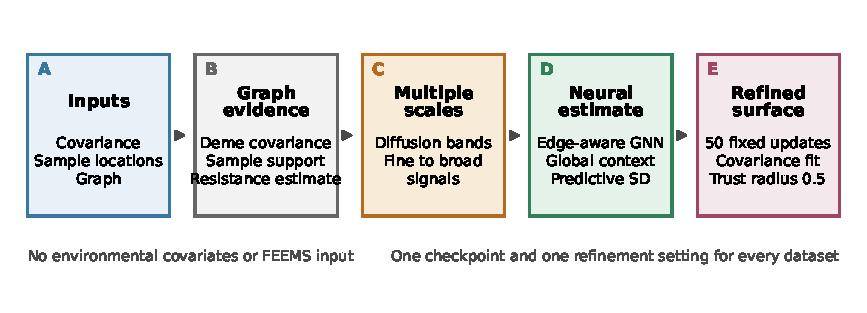
\includegraphics[width=\linewidth]{method_overview.pdf}
\caption{Overview of \dreems. Genetic covariance and sample locations are
placed on a user-supplied geographic graph. An all-pairs resistance
approximation and fixed diffusion bands provide edge and node features to a
graph neural network. The network predicts relative migration and uncertainty,
and a fixed trust-region step refines the surface against observed covariance.}
\label{fig:overview}
\end{figure}

\subsection{Training on simulated spatial histories}

We trained \dreems on 61,440 structured-coalescent simulations. The graphs
contained 9--1,743 nodes and included regular lattices, masked habitats,
corridors, and random windows sampled from landmasses around the world
(Table~\ref{tab:training-corpus}). Migration surfaces included homogeneous
isolation by distance, smooth heterogeneity, barriers, corridors, anisotropy,
coast effects, and variation in local drift. Sampling ranged from nearly full
coverage to a small fraction of graph nodes and was allowed to correlate with
the underlying migration process. Landscape variables generated the
simulation targets, but they were not model inputs.

Validation loss fell quickly during the first 10,000 updates and improved more
slowly thereafter (Figure~\ref{fig:training}). The lowest graph-balanced
validation loss occurred at step 29,000. Training stopped at step 41,000 after
12 further checks failed to improve the loss by the prespecified threshold,
and the step-29,000 parameters were restored. The separate set of 4,096
held-out examples was not used to select the checkpoint.

\begin{figure}[t]
\centering
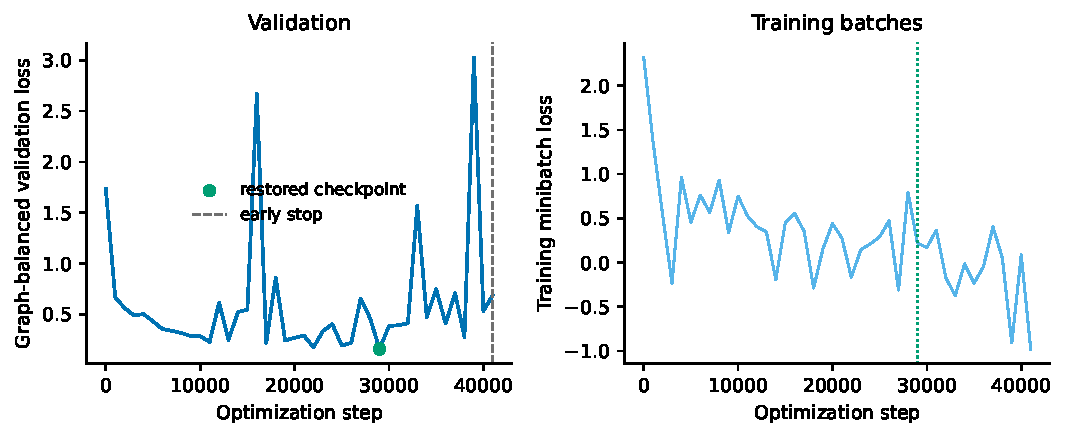
\includegraphics[width=0.92\linewidth]{training_curve.pdf}
\caption{Training of the production model. Validation loss was measured on
1,024 complete graphs at 1,000-step intervals. The green point marks the
restored checkpoint and the dashed line marks early stopping. Minibatch loss
is noisy because graph size and difficulty differ among batches.}
\label{fig:training}
\end{figure}

\subsection{DREEMS recovered simulated migration surfaces}

We generated 512 independent global-landscape examples for the main
comparison. These graphs contained 219--1,406 nodes and 590--4,065 edges. A
median of 39 graph nodes was observed, corresponding to a median sampled-node
fraction of 0.049. Each example contained a new graph window, migration
surface, sampling design, and structured-coalescent genotype simulation.

We ran \feems on the same genotype matrix, coordinates, and graph. For each
example, \feems jointly selected its migration and local-$q$ smoothing
parameters by documented leave-one-observed-deme-out cross-validation and
then refit the selected model to all samples. In contrast, \dreems used the
same checkpoint and radius-0.5 covariance refinement for all 512 examples.

Refined \dreems attained mean edge correlation 0.720 and mean squared error
(MSE) 0.533, compared with correlation 0.614 and MSE 0.738 for \feems
(Table~\ref{tab:h2h-overall}). Before refinement, the neural estimate had mean
correlation 0.698 and MSE 0.558. The fixed refinement therefore improved both
metrics without using the simulated truth to choose its radius.

The paired differences were also clear (Table~\ref{tab:h2h-paired}). Refined
\dreems increased mean correlation by 0.1058 (95\% CI 0.0897--0.1220) and
reduced mean MSE by 0.2048 (95\% CI 0.1773--0.2323) relative to \feems. It had
higher correlation in 419 of 512 examples (81.8\%) and lower MSE in 429
(83.8\%). The per-example comparison shows a broad shift rather than a small
number of large gains, although substantial \dreems failures remain
(Figure~\ref{fig:h2h-scatter}).

\begin{table}[t]
\centering
\caption{Graph-balanced mean performance on 512 independently generated
global-landscape examples. Covariance diagnostics were retained for \dreems
only.}
\label{tab:h2h-overall}
\small
\begin{tabular}{lrrrr}
\toprule
Method & Edge corr. & Edge MSE & Cov. corr. & Cov. R2 \\
\midrule
DREEMS neural & 0.698 & 0.558 & 0.939 & 0.917 \\
DREEMS refined & 0.720 & 0.533 & 0.984 & 0.976 \\
FEEMS documented LOO-CV & 0.614 & 0.738 & -- & -- \\
\bottomrule
\end{tabular}

\end{table}

\begin{table}[t]
\centering
\caption{Paired contrasts across the same examples. Positive advantage favors
the first method named. MSE advantage is baseline MSE minus candidate MSE.}
\label{tab:h2h-paired}
\scriptsize
\begin{tabular}{lrrrrr}
\toprule
Paired contrast & N & Mean advantage & 95\% CI & P & Win frac. \\
\midrule
Refined DREEMS vs FEEMS, correlation & 512 & 0.1058 & [0.0897, 0.1220] & 3.6e-33 & 0.818 \\
Refined DREEMS vs FEEMS, MSE & 512 & 0.2048 & [0.1773, 0.2323] & 9.6e-41 & 0.838 \\
Neural DREEMS vs FEEMS, correlation & 512 & 0.0835 & [0.0658, 0.1011] & 4.5e-19 & 0.711 \\
Neural DREEMS vs FEEMS, MSE & 512 & 0.1806 & [0.1499, 0.2112] & 9.8e-28 & 0.740 \\
Refinement vs neural, correlation & 512 & 0.0224 & [0.0128, 0.0319] & 5.4e-06 & 0.662 \\
Refinement vs neural, MSE & 512 & 0.0243 & [0.0140, 0.0345] & 4.3e-06 & 0.607 \\
\bottomrule
\end{tabular}

\end{table}

\begin{figure}[t]
\centering
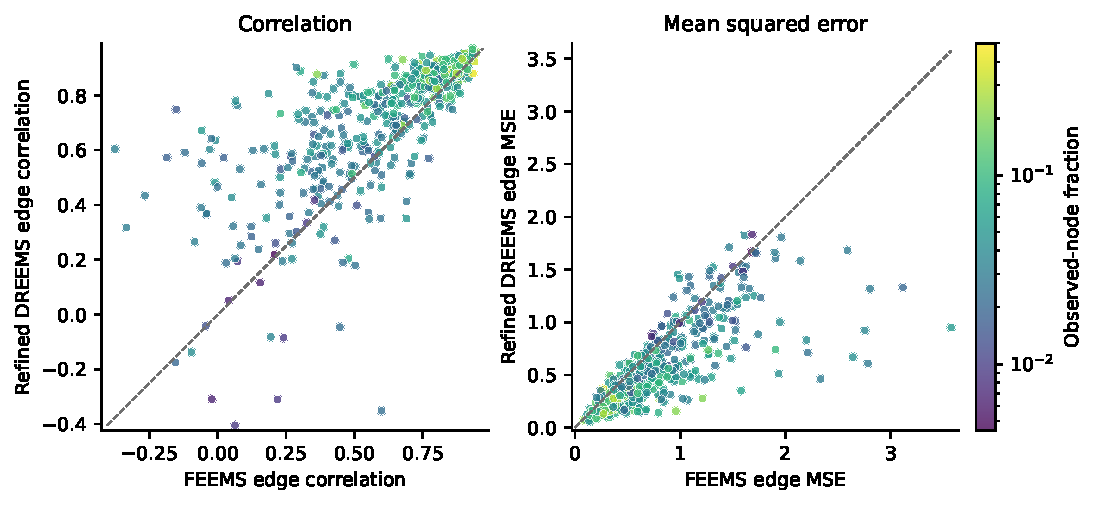
\includegraphics[width=0.94\linewidth]{h2h_scatter_corr_mse.pdf}
\caption{Recovery of simulated edge log-conductance. Each point compares
refined \dreems with documented \feems LOO-CV on one landscape. Points above
the diagonal in the correlation panel and below it in the MSE panel favor
\dreems. Color gives the fraction of graph nodes containing samples.}
\label{fig:h2h-scatter}
\end{figure}

The refinement had a larger effect on the quantity it directly targets. Mean
off-diagonal covariance correlation increased from 0.939 for the neural
surface to 0.984 after refinement, while mean covariance $R^2$ increased from
0.917 to 0.976. Mean edge correlation increased by 0.0224 and MSE decreased by
0.0243. Covariance fit and edge recovery are not equivalent: sparse
observations can be explained by more than one conductance surface.

Accuracy improved as more of the graph was sampled. Refined \dreems mean
correlation was 0.690 in the 430 sparse examples, 0.874 in 73 intermediate
examples, and 0.904 in nine dense examples
(Table~\ref{tab:h2h-regimes}). Nevertheless, its group mean exceeded \feems in
all three strata. In the sparse group, \dreems increased mean correlation by
0.1146 and reduced mean MSE by 0.2163. The dense stratum is too small for a
precise separate comparison.

The average \dreems advantage was also present in each graph-size stratum
(Table~\ref{tab:h2h-sizes}; Figure~\ref{fig:h2h-regimes}). The mean correlation
advantages were 0.1315 for graphs with 219--450 nodes, 0.0772 for graphs with
451--900 nodes, and 0.0860 for graphs with 901--1,406 nodes. Thus accuracy did
not collapse at the largest benchmark size, although all test graphs remained
within the training range.

\begin{table}[t]
\centering
\caption{Accuracy by observed-node fraction. D denotes refined \dreems and F
denotes documented \feems LOO-CV.}
\label{tab:h2h-regimes}
\scriptsize
\begin{tabular}{lrrrrrrr}
\toprule
Sampling & N & D corr. & F corr. & Corr. adv. & D MSE & F MSE & MSE adv. \\
\midrule
Sparse <=10\% & 430 & 0.690 & 0.575 & 0.1146 & 0.583 & 0.800 & 0.2163 \\
Intermediate 10-25\% & 73 & 0.874 & 0.811 & 0.0634 & 0.273 & 0.423 & 0.1507 \\
Dense >25\% & 9 & 0.904 & 0.873 & 0.0316 & 0.255 & 0.351 & 0.0956 \\
\bottomrule
\end{tabular}

\end{table}

\begin{table}[t]
\centering
\caption{Accuracy by graph size. Advantages are paired graphwise means.}
\label{tab:h2h-sizes}
\scriptsize
\begin{tabular}{lrrrrrrr}
\toprule
Nodes & N & D corr. & F corr. & Corr. adv. & D MSE & F MSE & MSE adv. \\
\midrule
219-450 & 252 & 0.664 & 0.532 & 0.1315 & 0.637 & 0.870 & 0.2329 \\
451-900 & 150 & 0.765 & 0.688 & 0.0772 & 0.436 & 0.604 & 0.1679 \\
901-1,406 & 110 & 0.786 & 0.700 & 0.0860 & 0.428 & 0.619 & 0.1908 \\
\bottomrule
\end{tabular}

\end{table}

\begin{figure}[t]
\centering
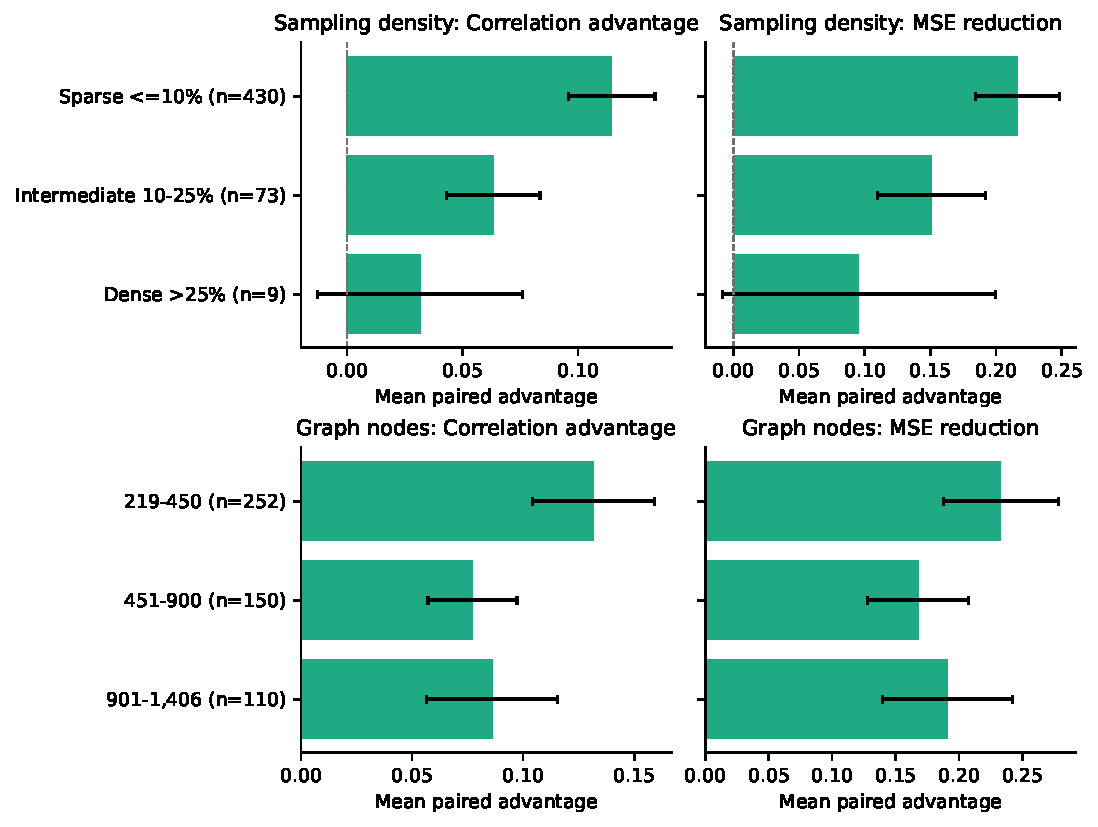
\includegraphics[width=0.94\linewidth]{h2h_regime_delta_bars.pdf}
\caption{Mean paired \dreems advantage by sampling and graph-size regime.
Positive values favor refined \dreems for both correlation and MSE reduction.
Bars show means and error bars show 95\% confidence intervals. The number of
graphs differs substantially among strata.}
\label{fig:h2h-regimes}
\end{figure}

Random examples show that both methods often recovered the largest
landscape-scale barriers (Figure~\ref{fig:h2h-random}). \dreems surfaces were
generally smoother and had lower amplitude. In many cases only a small
fraction of nodes was observed, so estimates across broad unsampled regions
were driven largely by resistance structure and the learned simulation prior.

The examples with the largest \dreems MSE disadvantage show its remaining
failure modes (Figure~\ref{fig:h2h-worst}). These include misplaced barriers,
excessive shrinkage, and incorrect extrapolation through sparsely sampled
regions. They are not merely sign-flipped versions of the truth. Because
empirical datasets provide no edge truth, such failures cannot be identified
by an oracle selector at prediction time.

\begin{figure}[p]
\centering
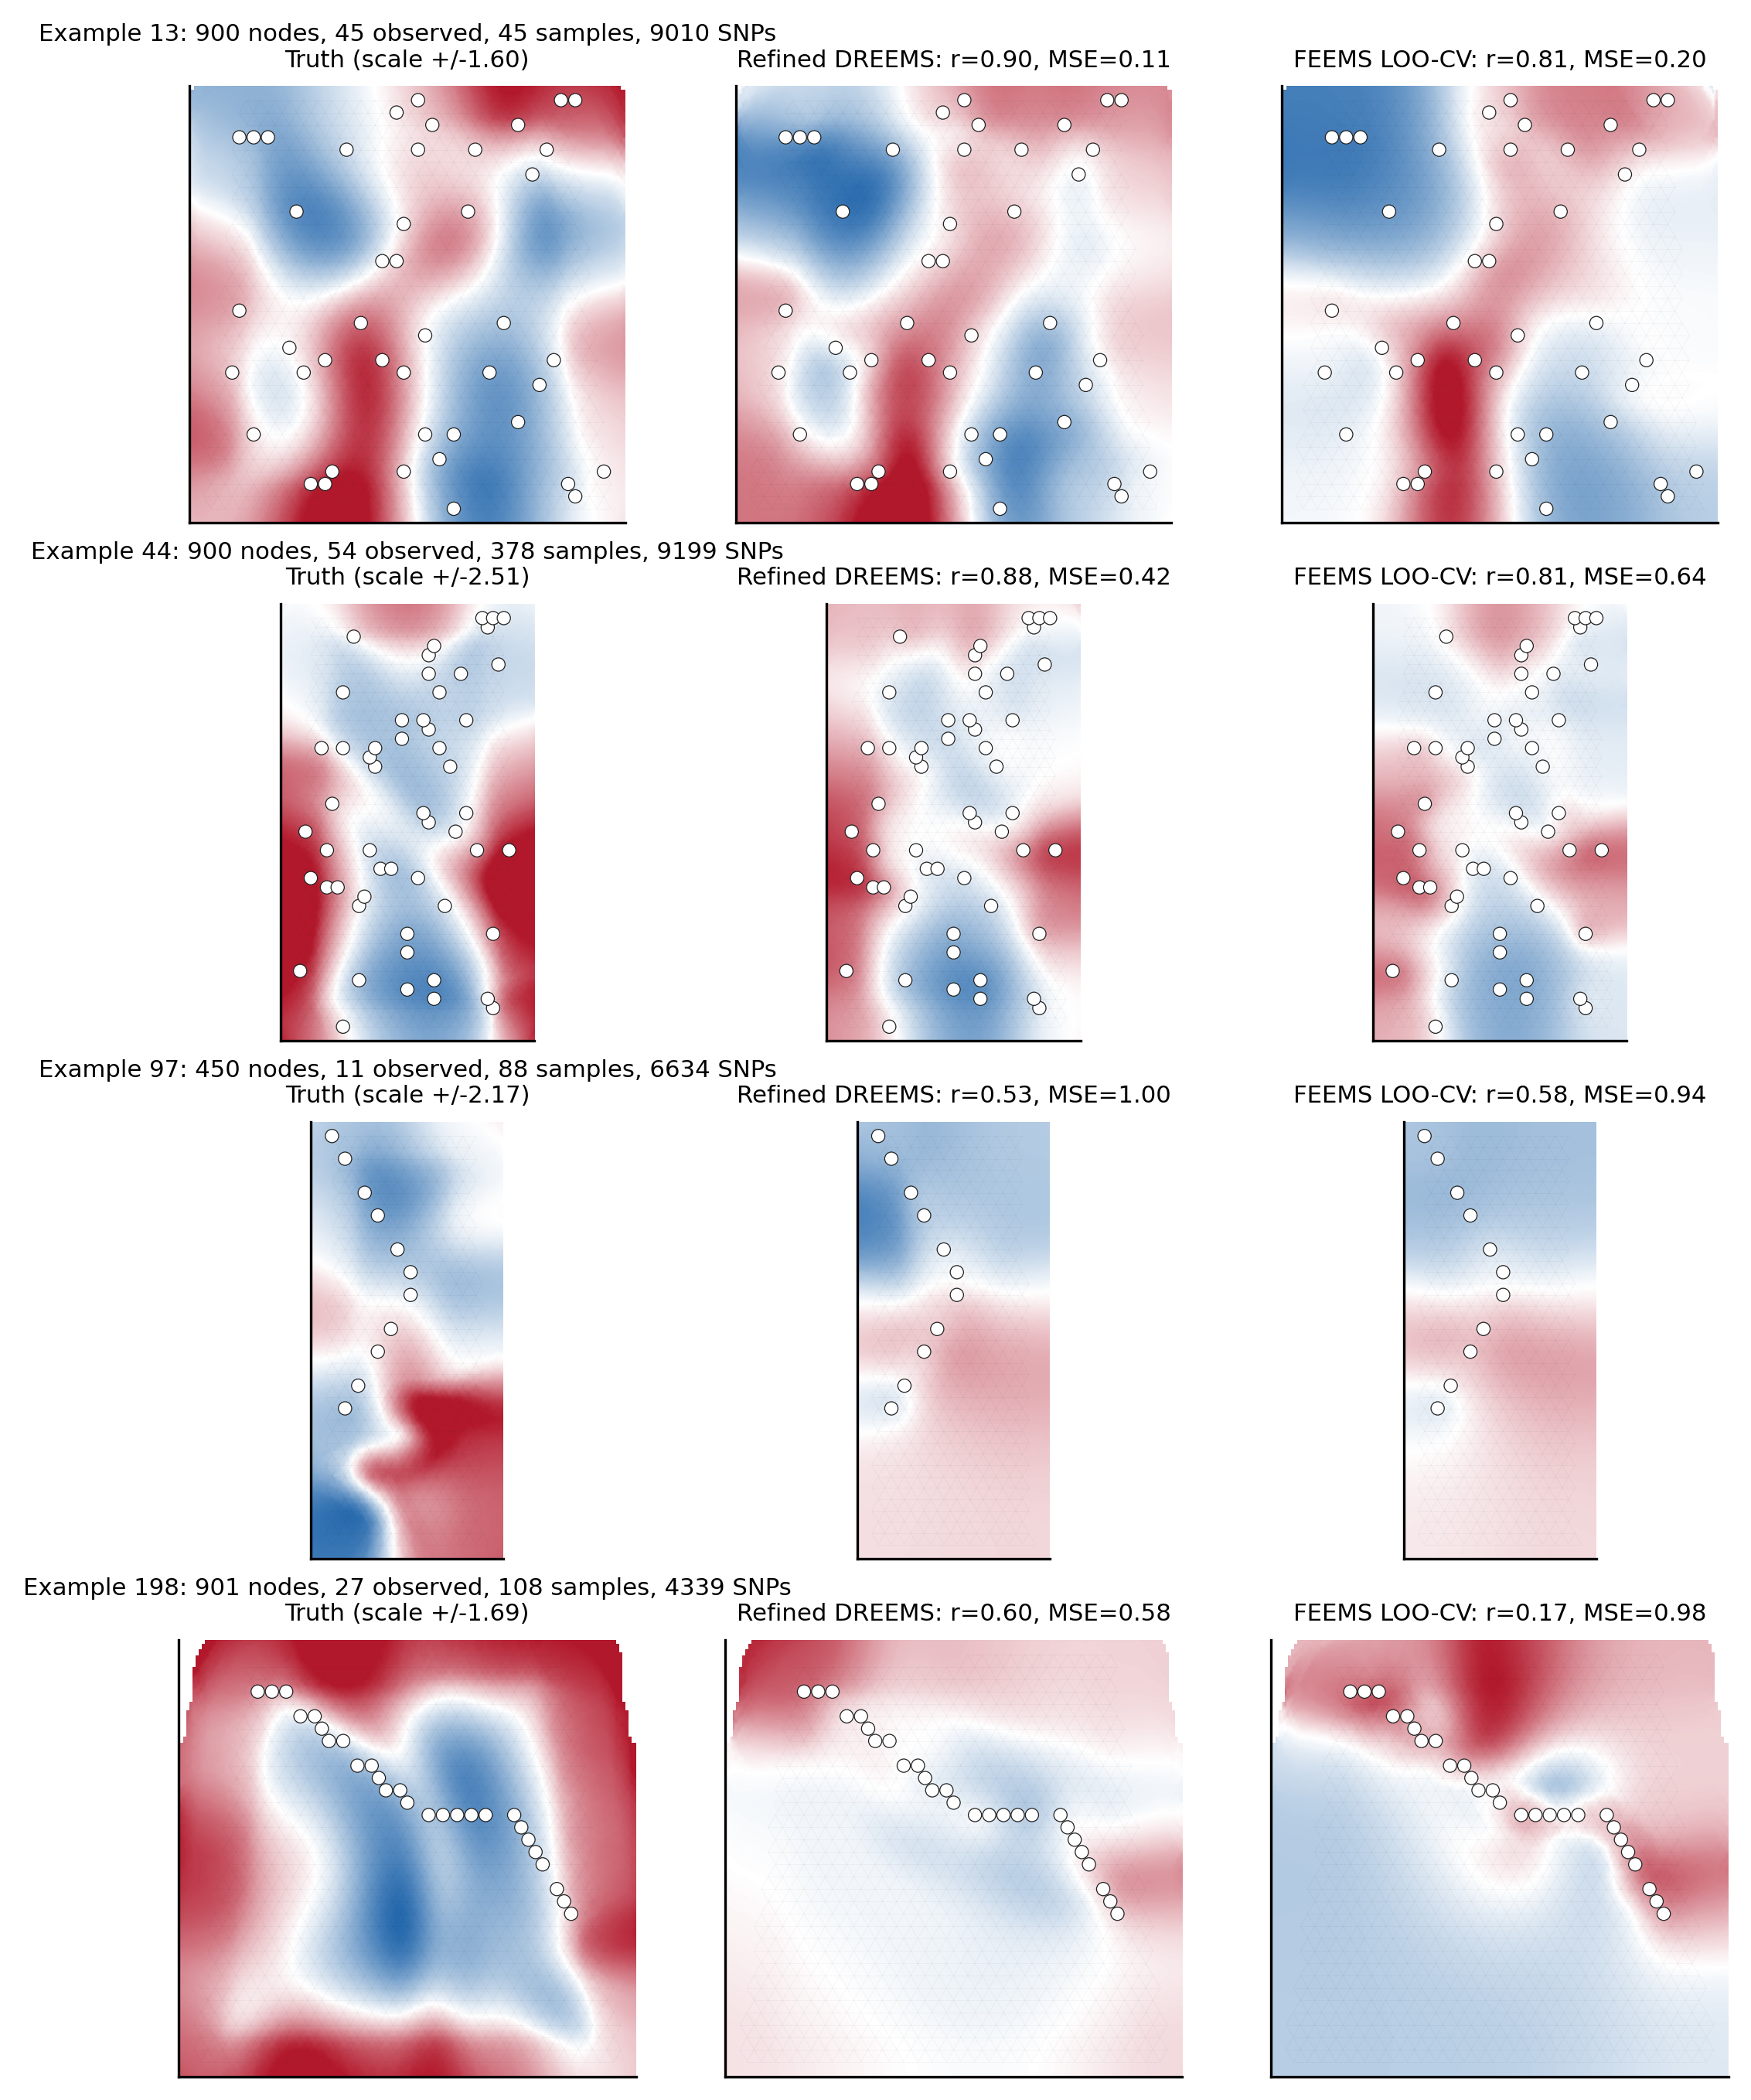
\includegraphics[width=\linewidth]{h2h_examples_random.png}
\caption{Random examples from the 512-landscape benchmark. Each row shows the
true surface, refined \dreems estimate, and \feems estimate on one centered
edge-log scale. Circles mark sampled nodes.}
\label{fig:h2h-random}
\end{figure}

\begin{figure}[p]
\centering
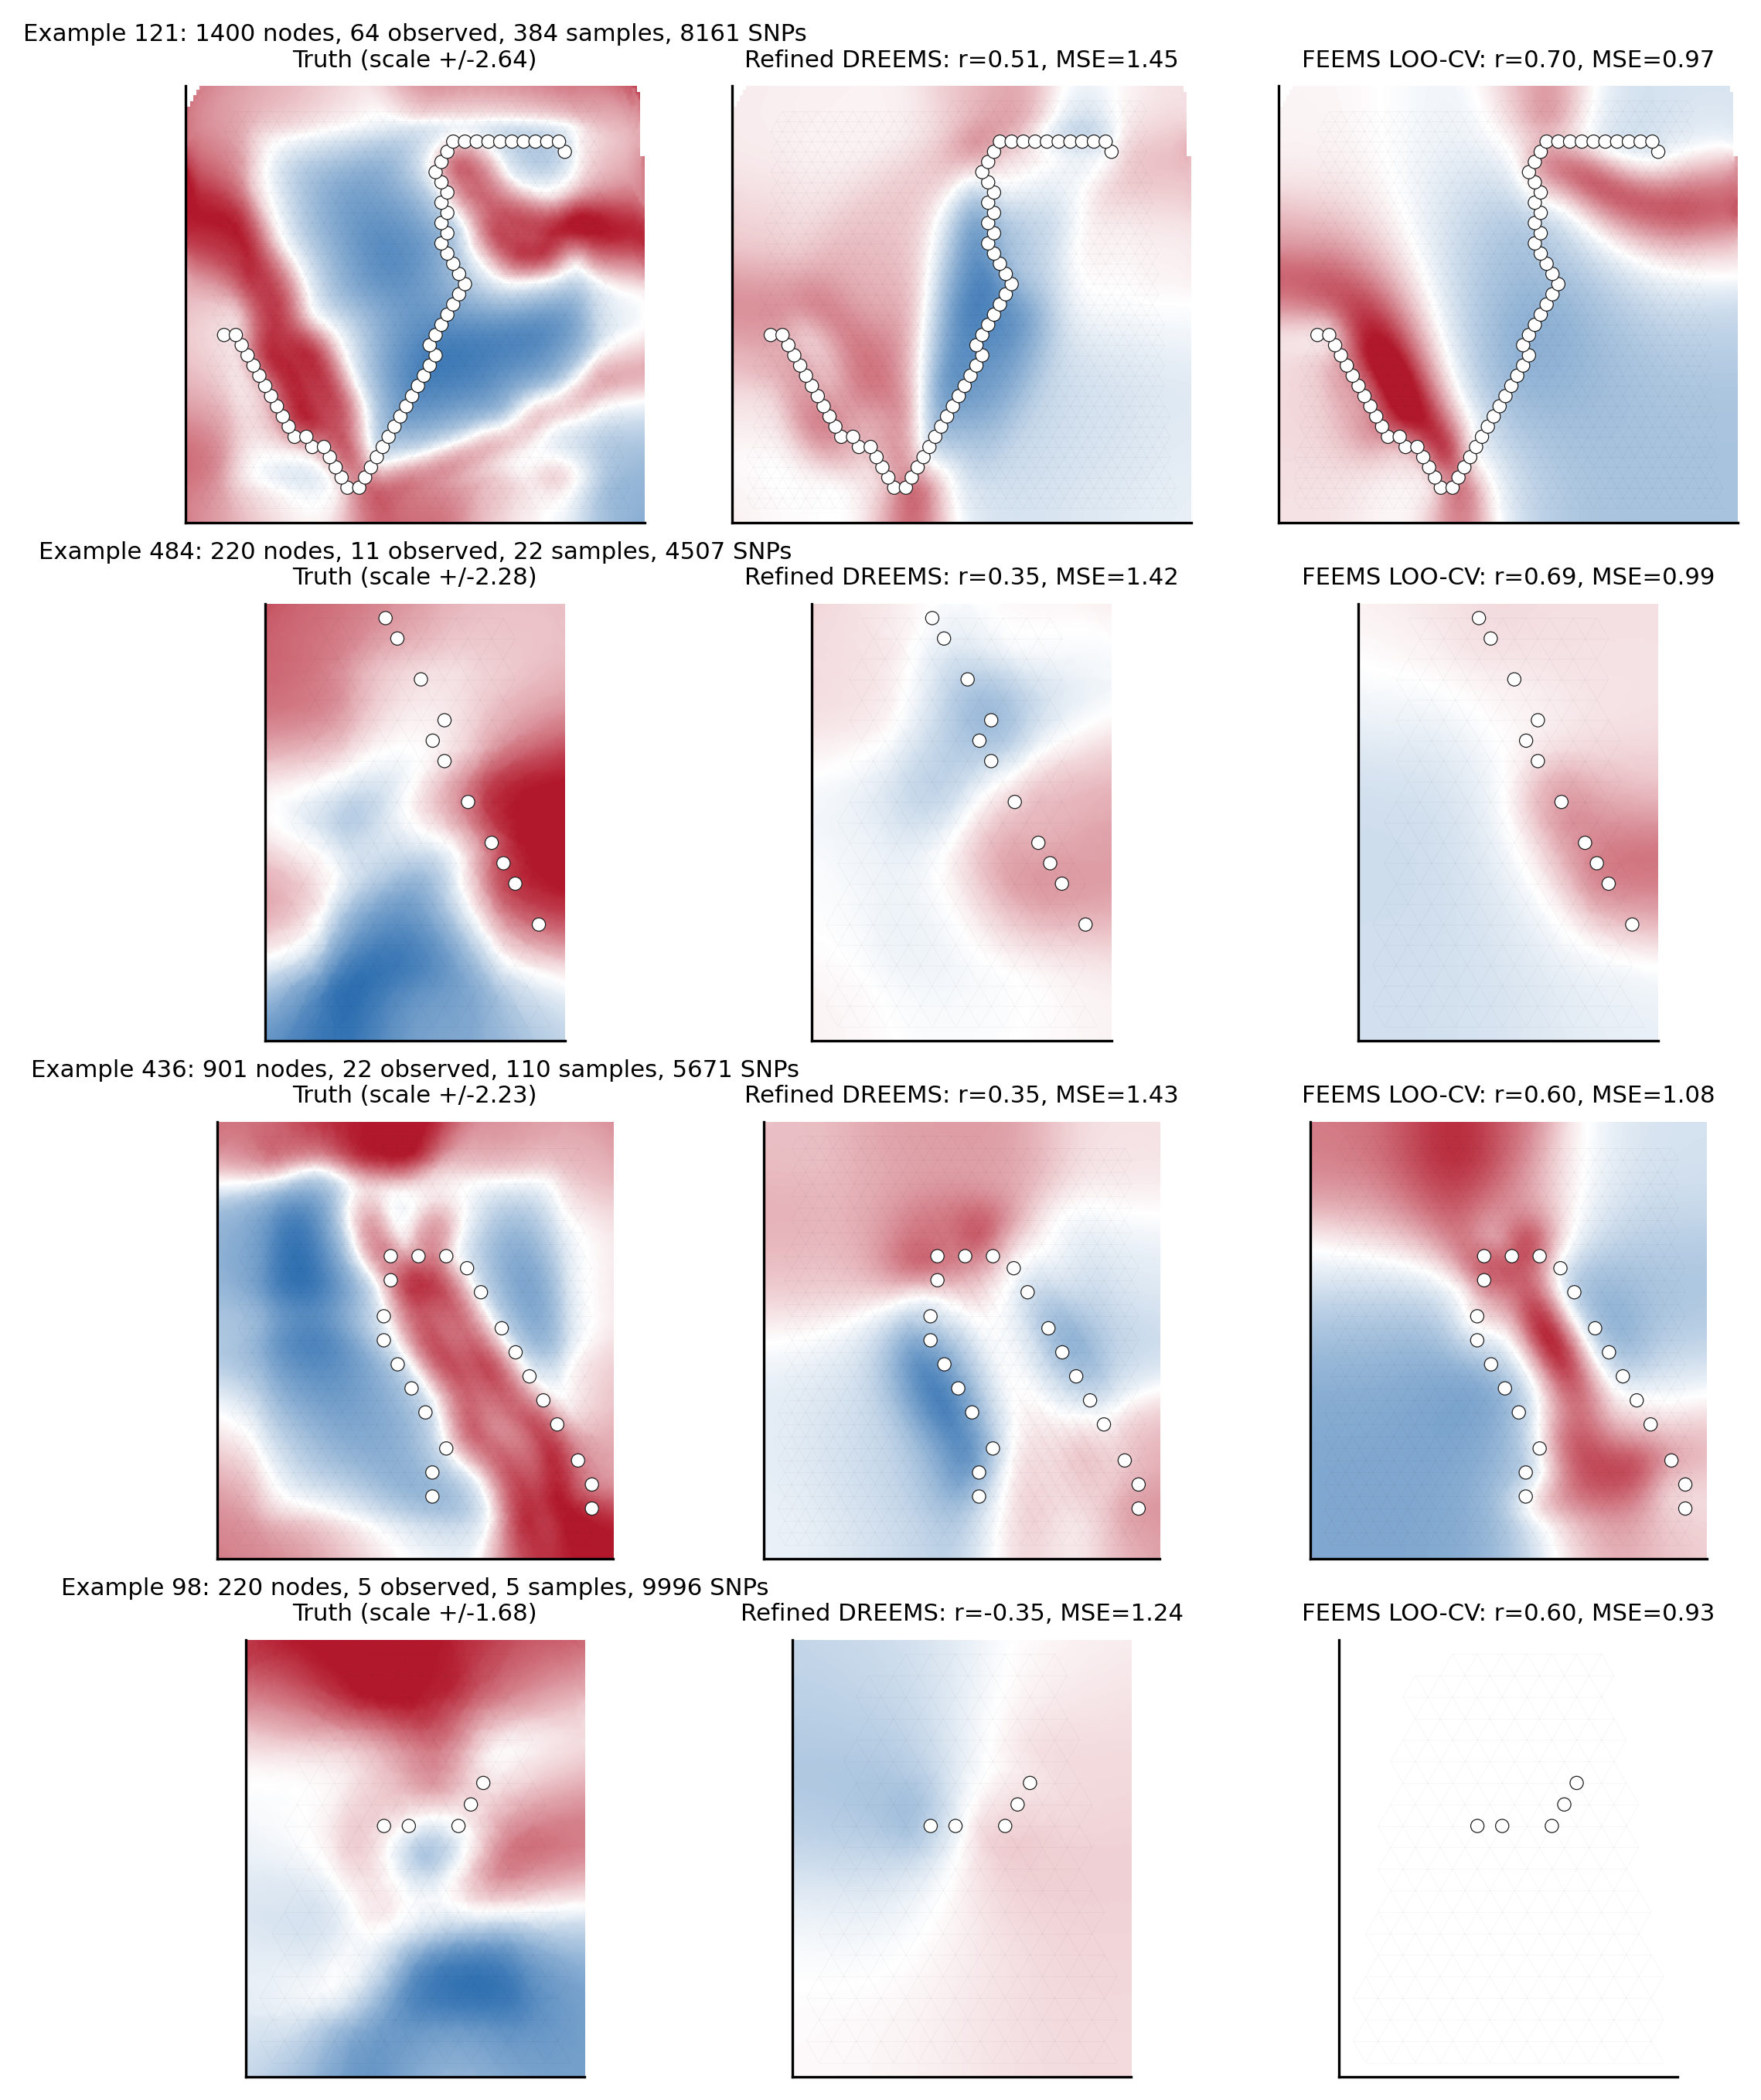
\includegraphics[width=\linewidth]{h2h_examples_worst_mse.png}
\caption{Examples with the largest MSE disadvantage for refined \dreems. This
deliberately unfavorable selection illustrates failure modes and does not
summarize average performance.}
\label{fig:h2h-worst}
\end{figure}

\subsection{DREEMS reduced the cost of repeated analyses}

Across 511 process-pool benchmark cases, median complete \dreems time was
8.4 s and the 95th percentile was 25.8 s. Median \feems LOO selection plus
final refit was 151.6 s and its 95th percentile was 1,365.6 s
(Table~\ref{tab:runtime}). The median paired runtime ratio was 16.4 and the
geometric mean ratio was 14.8. These timings favor \feems computationally:
its folds used a process pool of up to 16 workers, whereas \dreems used two
CPU threads. Even so, \feems runtime increased sharply with the number of
observed demes because each deme creates another cross-validation fold
(Figure~\ref{fig:runtime}).

One example with 384 observed demes was run with a separate Snakemake job for
every fold. Its ideal compute critical path was 333.9 s, but the folds used
75,904.9 aggregate CPU-seconds before the final refit
(Table~\ref{tab:runtime-atomized}). Parallel execution can reduce latency, but
it does not remove the computational work of cross-validation.

\begin{table}[t]
\centering
\caption{Executed runtime protocols for the 511 process-pool cases.
Parallelism was not matched and favors \feems.}
\label{tab:runtime}
\small
\begin{tabular}{lrlrr}
\toprule
Execution & N & Parallelism & Median s & P95 s \\
\midrule
DREEMS, complete refined estimate & 511 & 2 threads & 8.4 & 25.8 \\
FEEMS LOO-CV and final fit & 511 & up to 16 workers & 151.6 & 1365.6 \\
\bottomrule
\end{tabular}

\end{table}

\begin{table}[t]
\centering
\caption{Resource accounting for the separately atomized 384-fold \feems
example. Worker-seconds sum wall time over concurrent jobs.}
\label{tab:runtime-atomized}
\small
\begin{tabular}{lrrrr}
\toprule
Stage & Jobs & Critical path s & Worker-s & CPU-s \\
\midrule
FEEMS LOO folds & 384 & 269.2 & 83788.4 & 75904.9 \\
FEEMS selected final fit & 1 & 64.7 & 64.7 & 43.1 \\
Combined & -- & 333.9 & 83853.1 & 75948.0 \\
\bottomrule
\end{tabular}

\end{table}

\begin{figure}[t]
\centering
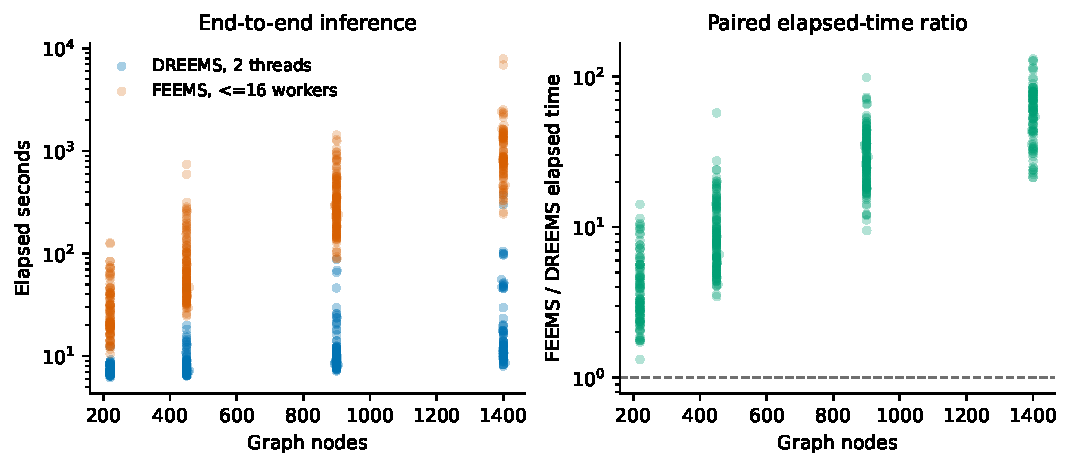
\includegraphics[width=0.94\linewidth]{runtime_scaling.pdf}
\caption{Measured runtime for the process-pool benchmark cases. Complete
elapsed time is shown against graph size (left), together with the paired
\feems-to-\dreems runtime ratio (right).}
\label{fig:runtime}
\end{figure}

\subsection{Predictive uncertainty identified difficult graphs}

We calibrated the network's predictive standard deviation on independent
simulations. On a separate 1,024-graph verification set, graph-balanced
coverage was 0.600, 0.857, and 0.957 for nominal 50\%, 80\%, and 95\%
intervals (Table~\ref{tab:calibration}). The 95\% interval was close to nominal
for sparse (0.951) and intermediate (0.949) graphs and conservative for the
dense group (0.983). The lower-level intervals overcovered overall.

Predictive SD was most informative about broad difficulty
(Table~\ref{tab:uncertainty}; Figure~\ref{fig:calibration}). Mean SD across a
graph had Spearman correlation 0.730 with graph MSE. At the edge level, SD had
pooled correlation 0.355 with absolute error. Mean within-graph correlation
was 0.203 and was positive in 86.3\% of graphs. Edge MSE increased from 0.127
in the lowest-SD quintile to 0.955 in the highest. The uncertainty estimate
therefore distinguishes easy from difficult graphs better than it pinpoints
every erroneous edge.

The covariance refinement changes the point estimate but does not update the
network SD. On the 512-landscape benchmark, centering the calibrated intervals
on the refined estimate gave 50\%, 80\%, and 95\% coverage of 0.579, 0.856,
and 0.963. These remain predictive intervals learned from simulations, not a
posterior distribution conditional on the refinement objective.

\begin{table}[t]
\centering
\caption{Marginal predictive-interval coverage. Verification graphs were not
used to fit or select the calibrator.}
\label{tab:calibration}
\small
\begin{tabular}{lrrrr}
\toprule
Evaluation & Graphs & 50\% & 80\% & 95\% \\
\midrule
Independent verification: all & 1024 & 0.600 & 0.857 & 0.957 \\
Independent verification: sparse <=10\% & 610 & 0.554 & 0.833 & 0.951 \\
Independent verification: medium 10-25\% & 211 & 0.590 & 0.842 & 0.949 \\
Independent verification: dense >25\% & 203 & 0.750 & 0.944 & 0.983 \\
Landscape H2H: neural & 512 & 0.564 & 0.846 & 0.958 \\
Landscape H2H: refined mean, neural SD & 512 & 0.579 & 0.856 & 0.963 \\
\bottomrule
\end{tabular}

\end{table}

\begin{table}[t]
\centering
\caption{Association between calibrated predictive SD and refined edge error
on 1,056,285 edges from the 512 global-landscape examples.}
\label{tab:uncertainty}
\small
\begin{tabular}{lr}
\toprule
Diagnostic & Value \\
\midrule
Pooled SD vs absolute refined error, Spearman & 0.355 \\
Mean within-graph Spearman & 0.203 \\
Graphs with positive within-graph association & 0.863 \\
Mean SD vs graph MSE, Spearman & 0.730 \\
Lowest-SD / highest-SD quintile MSE & 0.127 / 0.955 \\
\bottomrule
\end{tabular}

\end{table}

\begin{figure}[t]
\centering
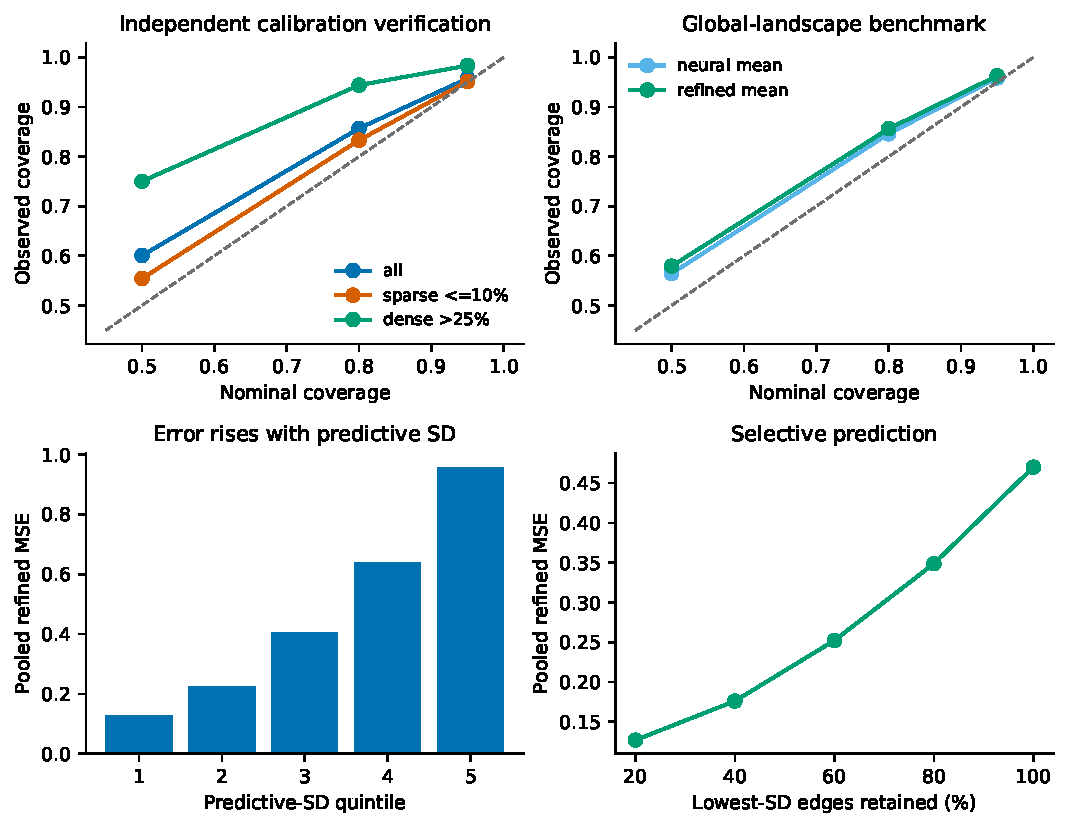
\includegraphics[width=0.94\linewidth]{calibration_utility.pdf}
\caption{Calibration and utility of predictive SD. Coverage is averaged by
graph. Error summaries use the refined mean and the unchanged calibrated
neural SD.}
\label{fig:calibration}
\end{figure}

\subsection{Application to empirical datasets}

We applied the same checkpoint without retraining to 15 public datasets
(Table~\ref{tab:empirical}). They span vertebrates, invertebrates, and plants,
with graphs containing 193--4,371 nodes. Fourteen analyses completed in
7.3--16.3 s; the largest sampled-node case, horseweed with 281 observed nodes,
took 161.0 s. The resulting surfaces showed broad geographic structure and
localized low-conductance regions in several taxa
(Figure~\ref{fig:empirical-dreems}). Because the true migration surfaces are
unknown, these analyses establish that the interface and checkpoint operate
across diverse public data, not that each inferred feature is correct.

For six examples, we placed the \dreems result next to a published EEMS,
\feems, or study figure (Figure~\ref{fig:empirical-published}). Several broad
patterns were visually similar, but local structure and amplitude often
differed. These panels are qualitative: the original studies can use different
variant filters, graphs, regularization, models, and rendering. We therefore
do not report numerical comparisons with the published images.

\begin{table}[p]
\centering
\caption{Public empirical datasets analyzed with one checkpoint. Obs. is the
number of graph nodes containing samples.}
\label{tab:empirical}
\scriptsize
\begin{tabular}{lrrrrrr}
\toprule
Dataset & Samples & SNPs & Nodes & Obs. & Edges & Seconds \\
\midrule
Gray wolves & 111 & 17729 & 1207 & 94 & 3458 & 16.3 \\
I. scapularis & 517 & 9197 & 511 & 42 & 1463 & 8.9 \\
C. cearae & 61 & 13681 & 418 & 16 & 1183 & 8.5 \\
S. cearensis & 48 & 13423 & 359 & 16 & 1023 & 7.6 \\
P. mcallii & 42 & 3731 & 262 & 16 & 704 & 8.0 \\
Poplar & 434 & 20601 & 773 & 35 & 2232 & 8.4 \\
Allohistium & 97 & 3333 & 516 & 39 & 1444 & 9.4 \\
C. galerita & 88 & 5990 & 557 & 38 & 1491 & 7.9 \\
B. tryoni & 293 & 6540 & 193 & 27 & 539 & 7.3 \\
P. cinereus & 38 & 232 & 1192 & 38 & 3394 & 9.8 \\
H. hajarensis & 30 & 1113 & 998 & 18 & 2901 & 9.7 \\
H. luqueorum & 23 & 1170 & 999 & 10 & 2905 & 8.0 \\
R. forreri & 103 & 172 & 4371 & 29 & 12829 & 15.7 \\
E. canadensis & 639 & 5080 & 1374 & 281 & 4029 & 161.0 \\
S. cayana & 83 & 19031 & 791 & 49 & 2310 & 9.0 \\
\bottomrule
\end{tabular}

\end{table}

\begin{figure}[p]
\centering
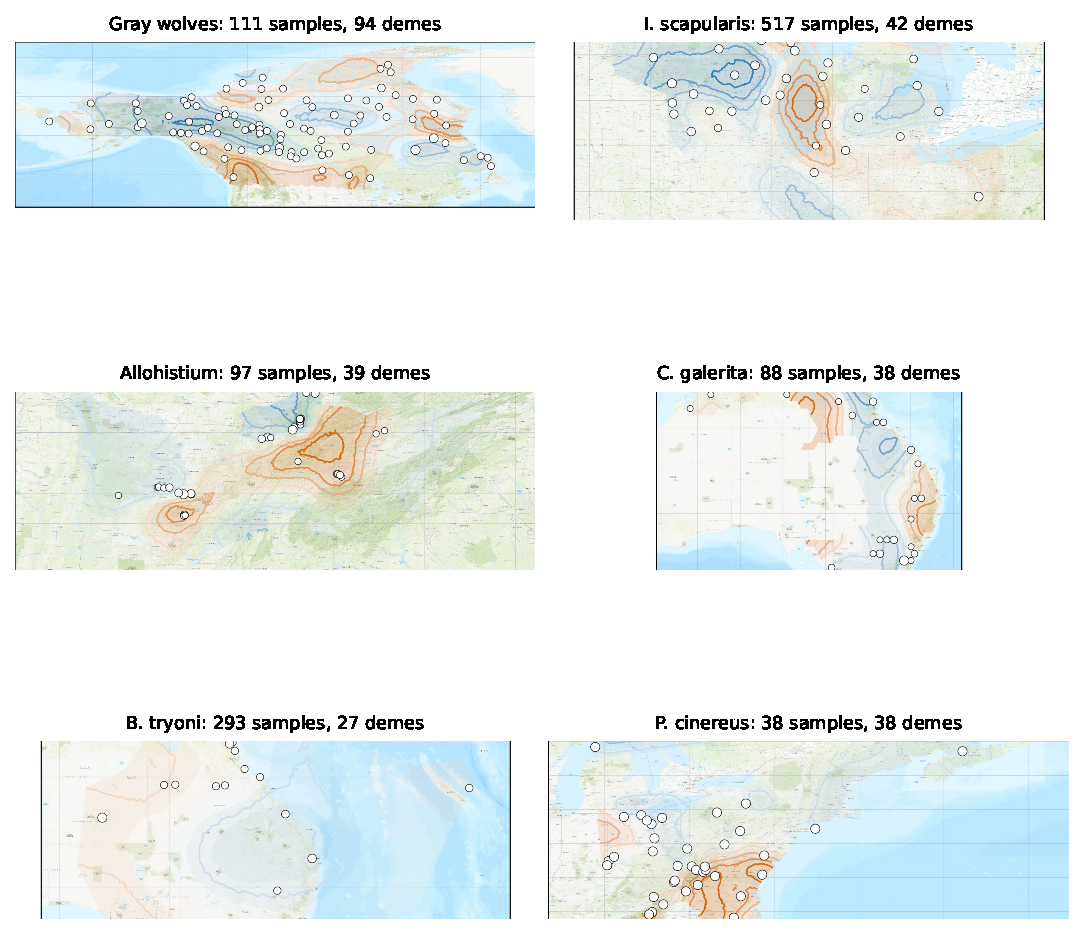
\includegraphics[width=\linewidth]{empirical_dreems_gallery.pdf}
\caption{Selected empirical \dreems surfaces. Blue indicates higher and red
lower centered relative migration; white is near the graph mean. Maps and
contours interpolate edge estimates for display only.}
\label{fig:empirical-dreems}
\end{figure}

\begin{figure}[p]
\centering
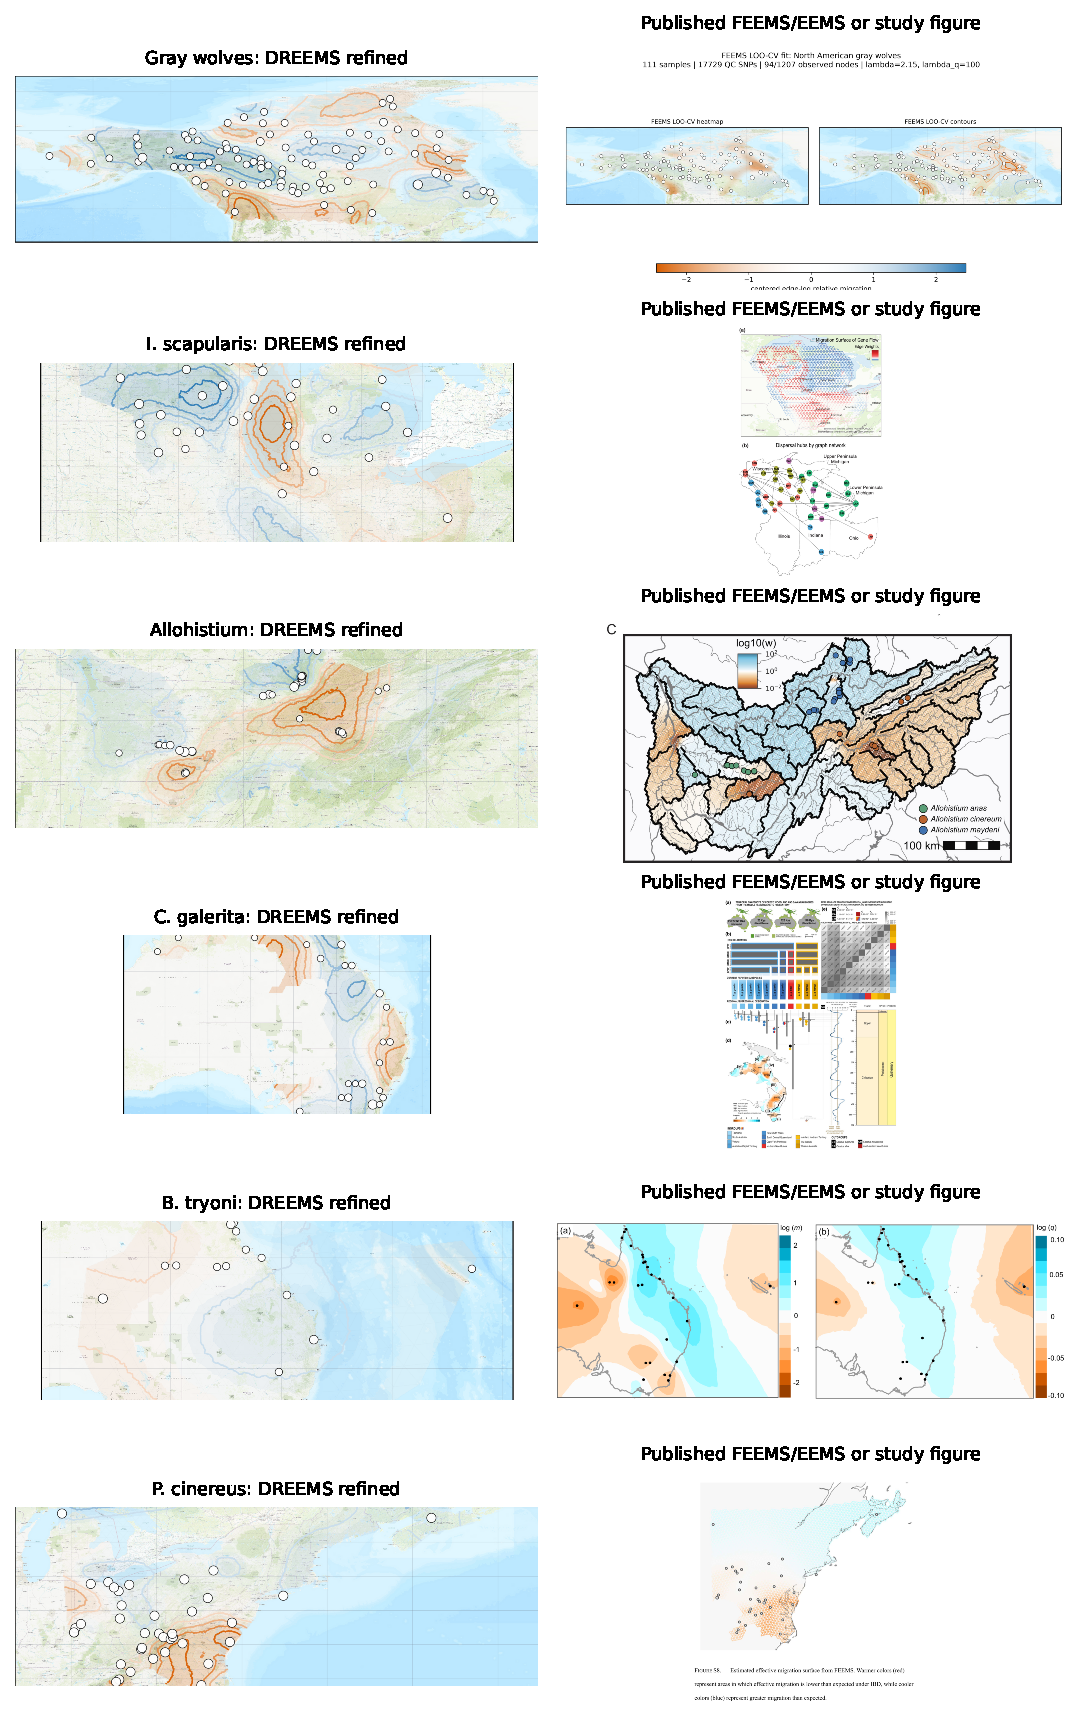
\includegraphics[width=\linewidth,height=0.82\textheight,keepaspectratio]{empirical_published_comparison.pdf}
\caption{Qualitative comparison with published FEEMS/EEMS or study figures.
Rows need not share graph, filtering, model, tuning, scale, or rendering, so
no numerical comparison is implied.}
\label{fig:empirical-published}
\end{figure}

\subsection{North American gray wolves exposed an empirical limitation}

The North American gray-wolf dataset provides a useful empirical test because
it was analyzed in the original \feems study and is distributed with its
software \citep{schweizer2016wolves,marcus2021feems}. The common-MAF-filtered
data contain 111 samples and 17,729 SNPs assigned to 94 of 1,207 graph nodes.
We ran \dreems and the documented 94-fold \feems procedure on this same graph
and genotype matrix.

The neural \dreems surface fit the off-diagonal covariance with correlation
0.672 and $R^2=0.477$. Refinement increased these values to 0.799 and 0.655.
\feems reached 0.892 and 0.775 (Table~\ref{tab:wolf}). The refined \dreems and
\feems edge fields had correlation 0.696, but the \dreems field had lower
edge-log standard deviation (0.784 compared with 1.131).

The difference is visible on the map (Figure~\ref{fig:wolf}). \feems placed a
strong low-conductance region across Hudson Bay and sharper contrasts along
coastlines. Refinement moved \dreems in the same direction relative to the
neural estimate, but its mean centered edge log-conductance in the broad
Hudson Bay region was $-0.074$, compared with $-0.557$ for \feems. The graph
size is within the training range, but only 7.8\% of nodes contain samples and
the real covariance need not follow the simulated demographic distribution.

\begin{table}[t]
\centering
\caption{North American gray-wolf diagnostics. Edge correlation is relative
to the \feems field, not to unknown truth. Hudson mean is a descriptive
centered edge-log average over a fixed bounding region.}
\label{tab:wolf}
\scriptsize
\begin{tabular}{lrrrrrr}
\toprule
Method & Cov. corr. & Cov. R2 & Cov. MSE & Edge corr. vs F & Edge SD & Hudson mean \\
\midrule
DREEMS neural & 0.672 & 0.477 & 0.001138 & 0.409 & 0.664 & 0.040 \\
DREEMS refined & 0.799 & 0.655 & 0.000751 & 0.696 & 0.784 & -0.074 \\
FEEMS 94-fold LOO-CV & 0.892 & 0.775 & 0.000489 & 1.000 & 1.131 & -0.557 \\
\bottomrule
\end{tabular}

\end{table}

\begin{figure}[t]
\centering
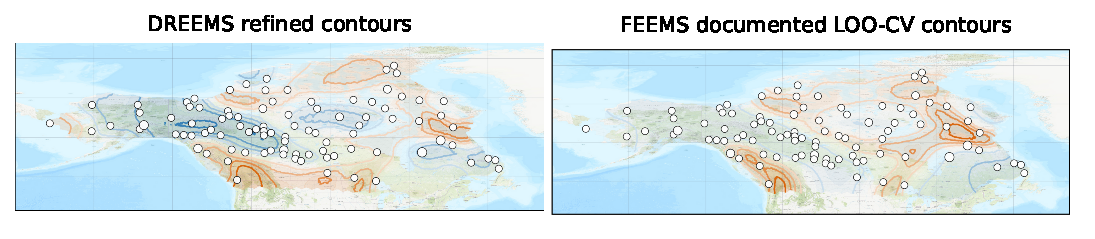
\includegraphics[width=\linewidth]{wolf_comparison.pdf}
\caption{North American gray-wolf surfaces using the packaged graph and the
same common-MAF-filtered data. Refined \dreems is shown at left and \feems,
selected by documented joint LOO cross-validation, at right.}
\label{fig:wolf}
\end{figure}

\clearpage
\section{Discussion}

\dreems provides a fast way to estimate effective migration surfaces from
genetic covariance. On 512 simulated landscapes, the refined estimate was
more accurate on average than \feems run with joint leave-one-deme-out
selection of migration and local-drift penalties. The advantage persisted in
the sparsely sampled group and across the tested range of graph sizes. Once
trained, one checkpoint could also be applied to 15 public datasets without a
new hyperparameter search.

The comparison measures two different ways of regularizing a difficult
inverse problem. \feems chooses a smooth surface separately for each dataset.
\dreems learns regularities across many simulated graphs and reuses them. More
than half of the training corpus was generated by the same global-landscape
meta-procedure as the synthetic benchmark, although every benchmark graph,
surface, sampling design, and random seed was new. The simulation result is
therefore evidence for amortization over this family, not a guarantee under an
arbitrary demographic model.

Several components helped make the learned estimate useful across graphs. The
linearized resistance calculation gives every observed pair a way to inform
edges that carry current between them. Diffusion bands retain genetic and
sampling patterns at several graph scales instead of relying only on repeated
local message passing. Graph-wide attention supplies long-range context. The
representation is also invariant to translation, rotation, reflection,
uniform scale, and node relabeling. This last property prevents the drawing of
a graph from creating a preferred migration direction.

The fixed covariance refinement combines the speed of a neural prediction
with a small amount of dataset-specific correction. It improved covariance fit
substantially and edge recovery modestly. The trust region is important because
many edge surfaces can explain a sparse observed covariance. Optimizing the
forward fit without this restriction can move toward a statistically similar
but spatially incorrect surface. Training through the refinement is possible
in principle, but would require a separate experiment to show that its added
cost improves generalization.

Predictive uncertainty supplies another diagnostic. After calibration, 95\%
marginal intervals had nearly nominal coverage on independent simulations,
and mean SD distinguished difficult from easy graphs. Local edge ranking was
weaker, and the factorized predictor does not describe dependence among edge
errors. The intervals also retain the neural SD after covariance refinement.
They should be read as simulation-based warning measures rather than Bayesian
credible intervals for an empirical dataset.

The wolf analysis illustrates the central limitation. \dreems was competitive
on the simulated landscape benchmark, yet \feems fit the empirical wolf
covariance better and recovered stronger structure around Hudson Bay. \dreems
receives no water or elevation layer, so it can recover a shoreline only when
genetic covariance, sample placement, graph geometry, and its learned prior
support that interpretation. The weaker wolf result suggests that this
combination of sparse sampling, geographic scale, and demographic history is
not fully represented by the training distribution.

Other limitations follow from the model itself. Relative effective migration
is not an identified contemporary migration rate. The present checkpoint
assumes a connected undirected graph, diploid simulations, and covariance from
common variants. It has not been validated for directional migration, strong
linkage, rare-variant summaries, polyploid genotypes, or graphs substantially
larger than those used in training. Interpolated maps can also appear more
continuous and geographically precise than the underlying edge estimates.

We therefore view \dreems as a rapid first analysis rather than a substitute
for scrutiny of the data and graph. Its clearest use is exploratory work across
many datasets or sensitivity analyses that would make repeated
cross-validation costly. For strong empirical claims, users should examine
covariance fit, predictive uncertainty, graph construction, and variant
filtering, and compare with a dataset-specific fit when the inferred surface
is unstable or biologically implausible.

\section{Materials and methods}

\subsection{Model description}

\paragraph{Migration as graph conductance.}
We represent a habitat by a connected, undirected graph $G=(V,E)$ with
$n=|V|$ nodes and $m=|E|$ edges. Let
$B\in\mathbb{R}^{m\times n}$ be an incidence matrix under an arbitrary edge
orientation. The target is a vector of relative edge log-conductances
$\vect{\theta}\in\mathbb{R}^m$. Positive conductances
$w_e=\exp(\theta_e)$ define the weighted graph Laplacian
\begin{equation}
    L(\vect{\theta})
    =B^\mathsf{T}\operatorname{diag}\{\exp(\vect{\theta})\}B.
    \label{eq:weighted-laplacian}
\end{equation}
The effective resistance between nodes $i$ and $j$ is
\begin{equation}
    R_{ij}(\vect{\theta})
    =
    (\vect e_i-\vect e_j)^\mathsf{T}
    L(\vect{\theta})^+
    (\vect e_i-\vect e_j),
    \label{eq:effective-resistance}
\end{equation}
where $L^+$ is the inverse on the mean-zero subspace. Multiplying every
conductance by the same constant changes the covariance scale but not the
relative surface. We therefore center true and estimated log-conductances to
have mean zero within each graph.

The canonical input is a node-level covariance matrix, coordinates for the
graph nodes, an undirected edge list, indices and sample counts for observed
nodes, and an effective SNP count. The public interface also accepts a sample
covariance matrix and sample coordinates, or genotypes and sample coordinates,
and constructs this object. Geographic coordinates assign samples to the
nearest node and determine normalized edge length. Environmental layers and a
fitted \feems surface are not inputs.

The model also predicts a centered node field
$\eta_i=\log q_i-\operatorname{mean}_j\log q_j$, where $q_i$ is the local
coalescence-rate coefficient used by the simulator. This nuisance output helps
the network distinguish variation in within-deme drift from edge conductance,
although the two remain statistically coupled.

\paragraph{Covariance calculation and deme aggregation.}
For a diploid genotype matrix $X$, with $s$ samples, $\ell$ SNPs, and entries
encoded as 0, 1, or 2, we remove monomorphic variants and standardize each
retained SNP across samples:
\begin{equation}
    Z_{al}
    =\frac{X_{al}-\bar X_{\cdot l}}
    {\operatorname{sd}(X_{\cdot l})},
    \qquad
    C=\ell^{-1}ZZ^\mathsf{T}.
    \label{eq:sample-covariance}
\end{equation}
The sample standard deviation uses denominator $s-1$. Missing genotypes in
the empirical analyses were mean-imputed after variant filtering. If $A$
averages samples assigned to each observed node, the node-level covariance is
$C_o=ACA^\mathsf{T}$.

When a user supplies covariance directly, we symmetrize it and project small
negative eigenvalues to zero before aggregation. The effective SNP count is
retained because it controls sampling-precision features. Covariance input
does not preserve linkage, allele-frequency spectra, or higher-order genotype
information.

\paragraph{Covariance score maps.}
We retain the leading 20 eigenpairs of the observed-node covariance and form
score maps
\begin{equation}
    U_k=\sqrt{\lambda_k}\vect v_k,
    \qquad k=1,\ldots,20.
    \label{eq:covariance-scores}
\end{equation}
Scores at unobserved nodes are zero, eigenvector signs are fixed
deterministically, and unavailable components are zero-padded. These are
eigenvectors of genetic covariance, not graph-Laplacian eigenvectors.

\subsection{All-pairs linearized resistance initializer}

The $o$ observed demes provide $o(o-1)/2$ pairwise dissimilarities
\begin{equation}
    D_{ij}=C_{o,ii}+C_{o,jj}-2C_{o,ij}.
\end{equation}
The initializer uses every observed pair. Its implementation batch size of
256 limits working memory and does not subsample the data.

We define a fixed baseline conductance
$w_e^{(0)}=\operatorname{clip}(d_{\mathrm{med}}/d_e,0.25,4)$ from edge length.
Sparse grounded solves give baseline resistances $R_{ij}^{(0)}$ and node
potentials $\vect\phi_{ij}$ for unit current injected at $i$ and removed at
$j$. The first-order sensitivity of log resistance to edge log-conductance is
\begin{equation}
    A_{(ij),e}
    =
    \left.
    \frac{\partial\log R_{ij}}{\partial\theta_e}
    \right|_{\vect\theta^{(0)}}
    =-
    \frac{w_e^{(0)}\{(B\vect\phi_{ij})_e\}^2}
    {R_{ij}^{(0)}}.
    \label{eq:resistance-sensitivity}
\end{equation}
Thus a pair contributes to each edge carrying baseline electrical flow between
its endpoints.

Let $\vect r$ be the centered difference between observed and baseline log
dissimilarity. We accumulate $\vect g=A^\mathsf{T}\vect r$ and the diagonal
information approximation $h_e=\sum_{i<j}A_{(ij),e}^2$ without materializing
the dense sensitivity matrix. The update solves
\begin{equation}
    \left[
      \operatorname{diag}(\vect h+\rho)+0.01L_E
    \right]\vect\delta=\vect g,
    \label{eq:linearized-initializer}
\end{equation}
where $L_E$ is the unweighted line-graph Laplacian and $\rho$ is 0.001 times
the median positive diagonal information. We center and scale $\vect\delta$
to unit standard deviation. The field and a numerical-validity indicator are
the final two edge features. This is a one-step diagonal approximation. It is
evidence for the network to denoise rather than a stand-alone inverse
solution.

\subsection{Fixed diffusion-band features}

The spatial representation is unchanged by translating, rotating, reflecting,
uniformly rescaling, or relabeling the same graph. The network receives no
absolute coordinates or signed $x$/$y$ edge displacement. Coordinate slots
retained for checkpoint-shape compatibility are fixed at zero. Edge length is
divided by a graph-level reference length, endpoint sample-count and precision
features use symmetric means and absolute differences, and support is routed
over all shortest paths rather than one arbitrarily selected path.

For the multiscale features, the reference edge weight is
$a_e=\operatorname{clip}(d_{\mathrm{med}}/d_e,0.25,4)$. If $A_0$ and $D_0$
are the corresponding adjacency and degree matrices, the fixed normalized
Laplacian is
\begin{equation}
    L_0=I-D_0^{-1/2}A_0D_0^{-1/2}.
\end{equation}
This operator depends on graph topology and relative edge length, not on the
unknown migration surface. For a node-signal matrix $S$, we compute
$S_t=\exp(-tL_0)S$ at $t=(0.25,0.5,1,2,4)$ and form
\begin{equation}
 \begin{split}
    \Psi_0(S)&=S-S_{0.25},\\
    \Psi_k(S)&=S_{t_k}-S_{t_{k+1}},\quad k=1,\ldots,4,\\
    \Psi_5(S)&=S_{4}.
 \end{split}
 \label{eq:diffusion-bands}
\end{equation}
The bands retain changes removed at successive diffusion scales and a final
coarse component.

The diffusion input contains 13 standardized node signals: the first eight
covariance score maps, log sample count, a sampled-node indicator, total and
within-deme covariance support, and the covariance diagonal. Six bands give
78 node features. For each signal and band, we compute three symmetric edge
summaries: absolute endpoint contrast, log one plus squared contrast, and mean
endpoint absolute energy. These give 234 edge features. Base features add the
full 20 covariance scores, sample and SNP precision, covariance support,
normalized length, symmetric endpoint summaries, and shortest-path support.
The final arrays have 109 node and 253 edge columns, including the two
initializer columns. Training-corpus means and standard deviations normalize
each column, with a standard-deviation floor of 0.2.

\subsection{Graph neural network}

Table~\ref{tab:model-setup} summarizes the model. We implemented it with
Equinox and JAX \citep{jax2018,deepmind2020jax,equinox2021}. An affine GELU
layer embeds node features in 128 dimensions. Ten residual edge-aware
message-passing layers apply directed messages
\begin{equation}
    \vect m_{j\rightarrow i}^{(k)}
    =
    \vect h_j^{(k)}\odot
    \operatorname{sigmoid}(W_g^{(k)}\vect x_{ij})
    +\operatorname{GELU}(W_m^{(k)}\vect x_{ij}),
    \label{eq:edge-message}
\end{equation}
followed by a residual node update using the mean incoming message. A
three-layer context branch uses the same graph. No graph coarsening or pooling
is present in the released architecture.

For edge $(i,j)$, the decoder uses
\begin{equation}
    \vect u_{ij}
    =
    [\vect h_i+\vect h_j,
      |\vect h_i-\vect h_j|,
      \vect x_{ij}],
\end{equation}
which is symmetric in its endpoints. A query derived from $\vect u_{ij}$
attends to keys and values from all context-node embeddings, giving every edge
graph-wide context despite finite message-passing depth. Separate affine heads
predict an edge mean $\mu_e$ and log variance $\ell_e$, with
$\ell_e\in[-7,5]$, and analogous node-$q$ outputs. Edge means and node means
are centered within each graph.

The output family is a factorized normal distribution trained against
simulated targets. It approximates the conditional distribution induced by
the simulation corpus. It is not the result of variational inference for an
explicit per-dataset likelihood, and it does not represent covariance among
edge errors. We therefore call $\exp(\ell_e/2)$ the network predictive SD, not
a posterior SD.

\begin{table}[t]
\centering
\caption{Model and optimization settings for the production checkpoint.}
\label{tab:model-setup}
\small
\begin{tabular}{ll}
\toprule
Component & Setting \\
\midrule
Node / edge dimensions & 109 / 253 \\
Hidden channels & 128 \\
Local / context graph layers & 10 / 3 \\
Graph-wide attention & yes \\
Covariance score maps & 20 \\
Diffusion times & 0.25, 0.5, 1, 2, 4 \\
Spatial representation & topology and normalized edge length \\
Coordinate-frame invariant & translation, rotation, reflection, scale \\
Linearized initializer & all\_pair\_diagonal\_adjoint \\
Initializer pairs & all observed-deme pairs \\
Predictive family & factorized\_normal \\
Training examples & 61,440 \\
Validation / held-out examples & 1,024 / 4,096 \\
Best / final step & 29,000 / 41,000 \\
Best validation loss & 0.1572 \\
Optimizer / learning rate / batch & Adam / 5e-5 / 8 \\
\bottomrule
\end{tabular}

\end{table}

\subsection{Graph-balanced training objective}

Let $\theta_e^\star$ and $\eta_i^\star$ be centered simulation targets. The
principal edge term is the graphwise heteroscedastic Gaussian negative
log-likelihood
\begin{equation}
    \mathcal L_{\mathrm{edge}}
    =\frac{1}{2m}\sum_{e=1}^m
    \left[(\mu_e-\theta_e^\star)^2\exp(-\ell_e)+\ell_e\right].
    \label{eq:edge-nll}
\end{equation}
The node-$q$ head uses the same form. The full loss is
\begin{equation}
 \begin{split}
    \mathcal L={}&
    \mathcal L_{\mathrm{edge}}
    +0.5\mathcal L_{\mathrm{context}}
    +0.5\mathcal L_q\\
    &+0.25\mathcal L_{\mathrm{slope}}
    +0.20\mathcal L_{\mathrm{corr}}
    +0.35\mathcal L_{\mathrm{orientation}}.
 \end{split}
 \label{eq:total-loss}
\end{equation}
The context term is edge MSE from the auxiliary branch. The slope term is a
Huber loss on the within-graph regression slope relative to one, the
correlation term is $1-r$, and the orientation term penalizes failure to
separate above- and below-mean target edges. Shape terms are disabled when the
target's centered RMS is at most 0.05. Every component is reduced within each
graph before averaging over the minibatch, so a graph contributes one weight
regardless of its edge count. The training loss contains no resistance or
covariance-forward term.

\subsection{Synthetic training corpus}

\paragraph{Graphs, surfaces, and sampling.}
We generated 61,440 training examples, 1,024 validation examples, and 4,096
held-out examples with disjoint random seeds. Table~\ref{tab:training-corpus}
reports the realized training ranges. The corpus combines five graph families.

The largest component contains 34,605 random global-landscape examples. We
sample geographic windows over land between $55^\circ$S and $72^\circ$N from
Natural Earth 50-m polygons \citep{naturalearth}, project each window to a
local azimuthal-equidistant system, and place a hexagonal mesh over its full
bounding box. Water nodes remain in the graph but cannot be sampled. Target
sizes are 220, 450, 900, or 1,400 nodes. Conductance surfaces combine a random
smooth field, habitat mismatch, edge length, water and coast penalties, and a
randomly placed sinuous ridge. Coefficients, length scales, and final edge-log
standard deviation vary among examples. A separate smooth field generates
local $q$. Natural Earth and latent habitat variables generate targets and
sampling designs; they are never supplied to \dreems.

Another 12,256 examples use the $8\times12$ triangular lattice from \feems
simulations, with homogeneous, barrier, and anisotropic surfaces and either
full or approximately 20\% node sampling. A further 5,123 examples use land
or synthetic-corridor graphs with wolf-like sampling paths. The remaining
9,456 use masked grids and earth-like graphs with smooth, barrier,
Gaussian-process, or constant surfaces. Across global-landscape and wolf-like
examples, requested sampled-node fractions are 0.03, 0.05, 0.10, 0.25, or
0.50, weighted toward the sparse values. Each sampled node contains one to
eight diploid individuals, up to 384 total in those families. Other graph
families extend the realized range to 1,200 samples.

\begin{table}[t]
\centering
\caption{Realized production training corpus. Counts refer to graphs, not
SNPs.}
\label{tab:training-corpus}
\small
\begin{tabular}{ll}
\toprule
Corpus property & Value \\
\midrule
Total & 61,440 \\
Global landmass graphs & 34,605 \\
FEEMS triangular lattices & 12,256 \\
Wolf-like graphs & 5,123 \\
Masked grids and earth-like graphs & 9,456 \\
Nodes & 9-1,743 (median 450) \\
Edges & 12-4,107 (median 1,255) \\
Observed-node fraction & 0.002-1.000 (median 0.091) \\
Diploid samples & 2-1,200 (median 200) \\
Accepted SNPs & 2,000-10,000 (median 5,994) \\
Edge log-rate SD & 0.350-1.600 (median 0.976) \\
Node log-q SD & 0.000-0.900 (median 0.452) \\
Simulator & Rust structured coalescent \\
Ascertainment & random marker conditional on MAF >=0.05 \\
\bottomrule
\end{tabular}

\end{table}

\paragraph{Structured-coalescent SNP simulation.}
We wrote a Rust simulator for large stepping-stone models. Its state consists
of ancestral lineages and their current demes. If deme $i$ contains $k_i$
lineages, coalescence occurs there at total rate
$q_i k_i(k_i-1)/2$; each lineage moves from $i$ to $j$ at the specified edge
migration rate. Production rates are symmetric. Descendant sets are stored in
one or more 128-bit words, and random draws use Rust \texttt{SmallRng}.

For the production \texttt{conditioned\_random\_marker} scheme, we simulate a
genealogy and select a branch proportional to branch length, which is the
location distribution of a random infinite-sites mutation conditional on a
mutation occurring on that genealogy. We retain a marker only when its sample
allele frequency lies in $[0.05,0.95]$ and repeat until reaching the requested
number. Within demes, derived and ancestral haplotypes are randomly paired
without replacement to form diploid dosages. Accepted dosage columns are
standardized and accumulated directly into
Equation~\ref{eq:sample-covariance}; genotype matrices are not stored for the
training corpus. Examples contain 2,000--10,000 accepted SNPs.

We compared the Rust simulator with \texttt{msprime} on small graphs and with
symmetry and closed-form checks for the symmetric island model
\citep{baum2022efficient}. Tests compared allele counts, pairwise differences,
and covariance summaries over replicates.

\subsection{Optimization and checkpoint selection}

We used Adam with learning rate $5\times10^{-5}$, minibatch size 8, and global
gradient-norm clipping at one \citep{kingma2015adam}. Training sampled graphs
repeatedly rather than making one pass through the corpus. We evaluated all
1,024 validation graphs every 1,000 steps. After a 20,000-step warmup, early
stopping required an improvement greater than $10^{-4}$ within 12 validation
checks. The best graph-balanced validation loss was 0.15724 at step 29,000.
Training stopped at step 41,000 and restored the step-29,000 parameters. The
one-GPU run took 7,578.6 seconds (2.11 h), used 2,230.1 CPU-seconds, and reached
5.35 GiB resident memory. The checkpoint SHA-256 is
\texttt{f0b677d2cc028252002d15fac843ca7347b1b352eb2286a18bd202b724aa92b4}.

\subsection{Fixed q-aware trust-region covariance refinement}

The neural prediction is amortized and need not closely fit one dataset's
covariance. The default pipeline therefore applies a fixed 50-step refinement
without selecting a test-specific hyperparameter. Let
$P_o=I_o-\vect1\vect1^\mathsf{T}/o$ and let $G_o(\vect\theta)$ be the
observed-node submatrix of $L(\vect\theta)^+$. Define
\begin{equation}
    \bar C_o=P_oC_oP_o,
    \qquad
    \bar G_o(\vect\theta)=P_oG_o(\vect\theta)P_o.
\end{equation}
From the predicted node field we also form
\begin{equation}
    Q_o(\vect\eta)
    =\operatorname{diag}
      \left\{\frac{\exp(\eta_i)}{n_i}:i\text{ observed}\right\},
    \qquad
    \bar Q_o=P_oQ_oP_o,
\end{equation}
where $n_i$ is the number of samples at observed node $i$.

At every edge update, nonnegative least squares fits global scales
$\alpha,\beta\geq0$ for the migration and local-$q$ bases. The objective is
\begin{equation}
 \begin{split}
    \mathcal J(\vect\theta)
    ={}&
    \frac{1}{2\binom{o}{2}}
    \sum_{i<j}
    \left\{
      \bar C_{o,ij}
      -\alpha\bar G_{o,ij}(\vect\theta)
      -\beta\bar Q_{o,ij}
    \right\}^2\\
    &+\frac{10^{-4}}{2m}
      \vect\theta^\mathsf{T}L_E\vect\theta.
 \end{split}
 \label{eq:refinement-objective}
\end{equation}
Analytic gradients through sparse grounded solves avoid constructing $L^+$.
We use 50 Adam updates at learning rate 0.15. Edge batches of 256 control
working memory only.

The update remains in an uncertainty-scaled trust region around the neural
mean $\vect\mu$:
\begin{equation}
    \left[
      \frac{1}{m}\sum_{e=1}^m
      \left\{
        \frac{\theta_e-\mu_e}{\max(\sigma^{\mathrm{raw}}_e,0.25)}
      \right\}^2
    \right]^{1/2}
    \leq0.5.
    \label{eq:trust-region}
\end{equation}
The radius uses the raw neural SD because it was fixed before post-hoc
calibration. The locked configuration has no Gaussian-prior penalty; its
weight is zero. We therefore call the procedure constrained covariance
refinement rather than MAP. Refinement changes the point estimate but not the
reported predictive SD.

\subsection{Synthetic head-to-head benchmark}

\paragraph{Test examples.}
We generated 512 independent global-landscape examples with new random seeds.
Graphs contain 219--1,406 nodes (median 452) and 590--4,065 edges (median
1,270). They contain 2--384 observed nodes (median 39), 5--384 diploid samples
(median 135), and 2,003--9,996 accepted SNPs (median 5,811). The observed-node
fraction ranges from 0.004 to 0.500 (median 0.049). We evaluate both the frozen
neural mean and the fixed radius-0.5 refined mean.

\paragraph{Documented \feems LOO cross-validation.}
We pinned upstream \feems 2.0 at commit
\texttt{aa890b0e8ef583dd657a6a696af591b732d1d8be}. Following its documented
cross-validation notebook and source, each fold holds out all samples at one
observed deme. Candidate fits use the remaining demes, and selection scores
held-out allele-frequency prediction by L2 error. We jointly search ten
migration-smoothness values logarithmically spaced from 100 to 0.001 and five
$q$-smoothness values from 100 to 0.01. The selected pair is refit to all
samples with node-specific $q$, unbounded log weights, and at most 15,000
iterations. This gives \feems its documented leave-one-observed-deme-out,
dataset-specific selector; \dreems uses one checkpoint and one prespecified
refinement for every example. Both methods receive the same genotype matrix,
sample locations, and graph.

\paragraph{Accuracy and paired inference.}
For each graph, we center estimates and true edge log-conductances and compute
Pearson correlation and mean squared error (MSE). Each graph contributes one
value, regardless of edge count. For paired contrasts, an advantage is
\dreems correlation minus \feems correlation or \feems MSE minus \dreems MSE.
We report the mean advantage, a two-sided 95\% Student-$t$ interval, the paired
$t$-test $P$ value, and the fraction of examples won. Sampling strata are
sparse ($\leq10\%$ of graph nodes observed), intermediate ($>10\%$ and
$\leq25\%$), and dense ($>25\%$). Graph-size strata were fixed before
summarization.

For \dreems only, we also evaluate covariance fit by correlating observed
off-diagonal centered covariance with $\alpha\bar G_o+\beta\bar Q_o$ and by
its $R^2$ and MSE. Comparable covariance predictions were not retained in the
completed synthetic \feems artifacts, so these values are diagnostic rather
than a cross-method covariance comparison.

\subsection{Runtime and resource accounting}

Runtime includes model loading, feature construction, the neural forward pass,
and refinement for \dreems, and all LOO folds plus the selected final refit for
\feems. In 511 cases, \dreems used two CPU threads and \feems executed folds
through a process pool of up to 16 workers. The remaining example had 384
\feems folds, each represented as an independent Snakemake job
\citep{koster2012snakemake}; we report its idealized compute critical path and
aggregate worker use separately. These measurements describe the executed
workflows, not hardware-normalized single-core benchmarks. Training and
corpus-generation costs are not charged to an individual \dreems analysis.

\subsection{Predictive-SD calibration and utility}

We used three independent sets of 1,024 simulated graphs for calibration fit,
model selection, and verification. Candidate calibrators left raw SDs
unchanged, multiplied all SDs by one global scale, or applied additional
sampling-density factors for fractions $\leq0.10$, 0.10--0.25, and $>0.25$.
Parameters were fit by graph-balanced normal NLL, and the candidate with
lowest NLL on the selection set was locked. The selected density calibrator
had global multiplier 1.3117 and density factors 1.0753, 0.9951, and 1.9091.
We then measured graph-balanced 50\%, 80\%, and 95\% marginal coverage on the
verification set. The same locked calibration was used in the 512-example
head-to-head benchmark.

To ask whether uncertainty is useful beyond coverage, we correlated calibrated
edge SD with absolute refined error, computed within-graph rank correlations,
correlated graph-mean SD with graph MSE, and compared MSE across pooled SD
quintiles. These are marginal diagnostics for a factorized predictor, not
simultaneous coverage statements.

\subsection{Empirical reanalyses}

We applied the checkpoint without retraining to 15 public datasets that had
georeferenced genotypes, covariance-like EEMS input, or an existing
EEMS/\feems analysis. For raw genotypes we retained biallelic variants,
required study-appropriate call rate, mean-imputed missing calls, and applied a
common minor-allele-frequency threshold of 0.05. Exact source, filtering,
graph construction, and SNP-count provenance is stored per dataset in the
release manifest. Graphs contain 193--4,371 nodes and 539--12,829 edges;
observed fractions range from 0.0066 to 0.2045.

Published comparison panels were copied from the original papers or
author-distributed EEMS output. They can differ from our reanalysis in input
filtering, graph construction, regularization, method, and rendering. We use
them only for a qualitative visual audit. Because true conductance fields are
unknown in empirical data, no edgewise accuracy is reported.

The North American gray-wolf data distributed with \feems received a separate
same-graph analysis \citep{schweizer2016wolves,marcus2021feems}. The common-MAF
filtered matrix contains 111 samples and 17,729 SNPs assigned to 94 of 1,207
nodes on the packaged 3,458-edge graph. We compare neural and refined \dreems
with \feems selected by its 94-fold joint LOO procedure. As descriptive
diagnostics, we report off-diagonal covariance fit, correlation of each
\dreems edge field with the \feems field, edge-field standard deviation, and
mean centered edge log-conductance in a broad Hudson Bay bounding region. The
last quantity is not a formal geographic hypothesis test.


\section*{Data and code availability}

The software includes the Equinox checkpoint, an xarray-based Python API,
command-line entry points, the Rust simulator, tests, and Snakemake workflows
for corpus generation, training, calibration, \feems comparison, and figure
construction. The exact checkpoint SHA-256 is
\texttt{f0b677d2cc028252002d15fac843ca7347b1b352eb2286a18bd202b724aa92b4}.
The manuscript release manifest records hashes for the checkpoint, benchmark
rows, training history, calibration report, empirical provenance, tables,
figures, and PDF. Public-data source URLs and dataset-specific quality-control
steps are stored in the empirical manifest.

\bibliographystyle{plainnat}
\bibliography{references}

\end{document}
